\documentclass{article}
\usepackage[utf8]{inputenc}
\usepackage[spanish]{babel}
\usepackage{listings}
\usepackage{graphicx}
\graphicspath{ {images/} }
\usepackage{cite}
\usepackage{hyperref}

\begin{document}

\begin{titlepage}
    \begin{center}
        \vspace*{1cm}
            
        \Huge
        \textbf{Parcial 1 Informática II}
            
        \vspace{0.5cm}
        \LARGE
        Informa2 S.A.S
            
        \vspace{1.5cm}
            
        \textbf{Johan David Rojas\\Luis Fernando Torres\\Mateo Alejandro Bravo}
            
        \vfill
            
        \vspace{0.8cm}
            
        \Large
        Despartamento de Ingeniería Electrónica y Telecomunicaciones\\
        Universidad de Antioquia\\
        Medellín\\
        Abril de 2021
            
    \end{center}
\end{titlepage}

\tableofcontents
\newpage
\section{Análisis del problema}\label{analisis}
Para solucionar este desafio, se plantea un algoritmos que esta dividido en 2 etapas.

\begin{itemize}
    \item \textbf{Etapa de Software}\label{sw}
    En esta etapa se recopila toda la información que el usuario ingresa por el monitor serial para ser procesada en la siguiente etapa. Aquí se debe ingresar el patrón de caracteres que el usuario desea ver en la matriz de LEDs y se realiza el proceso de llevar cada carecter a un sistema binario que la electronica del montaje entienda, es decir se codifica la solicitud del usuario.

    \item \textbf{Etapa de Hardware}\label{hw}
    En esta etapa se cuenta con un arreglo asignado para cada carácter. En el montaje del circuito se tiene ocho 74HC595 (cada uno controla una fila de la matriz) conectados de tal forma que llevándole información por el puerto SER mostrará un patrón correspondiente al carácter ingresado por el monitor serial. Cada posicion del arreglo nos dará información del dato a llevar al circuito integrado. Por cada circuito integrado habrá ocho salidas que en total serán 64 salidas que determinarán el estado de los LED, a cada LED se le conecta un resistor para evitar daños. 

\end{itemize}
Una vez explicadas las etapas que se van a tener en cuenta en la solución de este desafío, se comienza a analizar la manera en la que se debe realizar el procedimiento para mostrar un solo carácter en el arreglo de LEDs, es decir como se va a implementar la función Imagen(). Para ello se realiza una recopilación de ideas, con posibles pasos que debe llevar cada etapa y unas observaciones para tener muy claro que se hace, tal como se muestra en la figura(\textbf{\ref{f1}}) :

    \begin{figure}[h]
    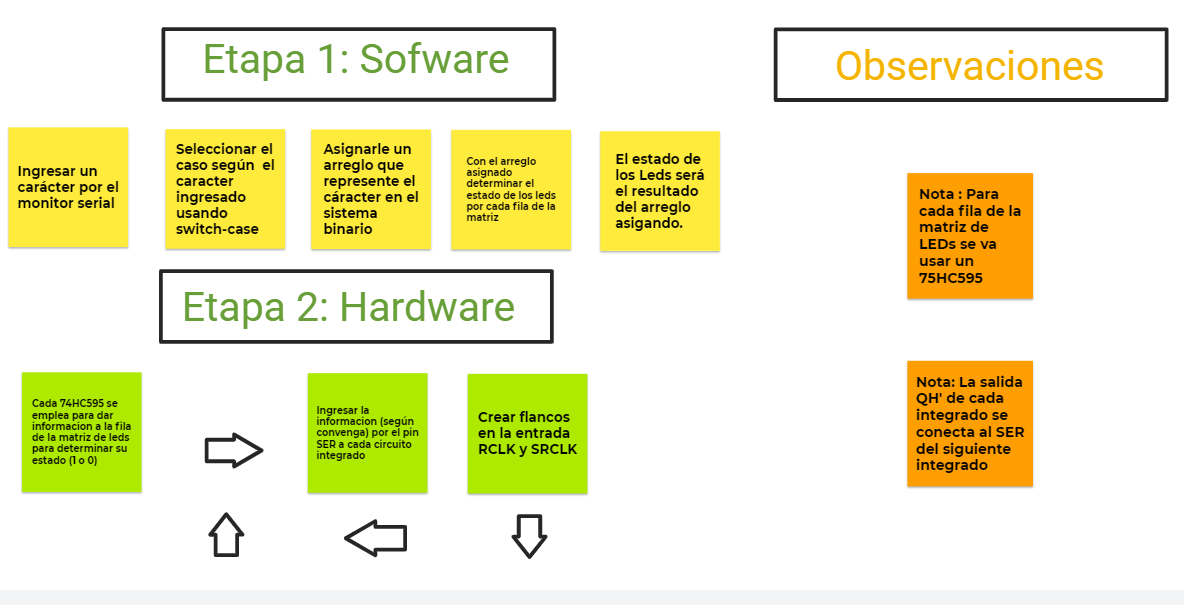
\includegraphics[width=12cm]{funimagen.png}
    \centering
    \caption{Procedimiento para mostrar un solo carácter}
    \label{f1}
    \end{figure}


\section{Proceso inicial de desarrollo} \label{desarrollo}
Para llevar a cabo la solución de este reto, lo que se busca es que el carácter que la persona ingrese por el monitor serial, sea reflejado en una matriz de LEDs y que se pueda observar de manera clara. Para ello se debe utilizar el sistema binario, ya que este indica el estado de un LED, donde cero (0) representa apagado y el uno (1) encendido.\\

Teniendo en cuenta lo dicho anteriormente, lo que se va a hacer es mostrar el carácter ingresado, en un arreglo de números en  sistema binario, indicando que LEDs deben encenderse para formar dicho patrón ingresado en la matriz. tal como se muestre en la figura(\textbf{\ref{A}}):


    \begin{figure}[h]
    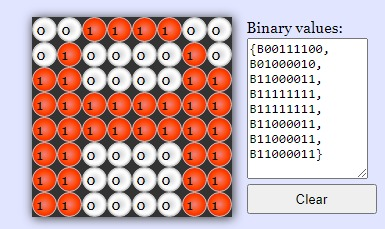
\includegraphics[width=8cm]{A.jpeg}
    \centering
    \caption{Letra A codificada para representar en la matriz}
    \label{A}
    \end{figure}

En la figura(\textbf{\ref{A}}), se puede observar el ejemplo con la letra A. En la matriz de LEDs que está ubicada en la parte izquierda, los números uno que están en color naranja, indican como se va a ver esta letra en la matriz real de LEDs. Por otra parte derecha muestra el arreglo que representa esta letra en sistema binario, el cual es el que se va a procesar por medio del integrado 74HC595. Para realizar este proceso de conversion se hizo uso de una herramineta online de mucha ayuda \cite{riyas}, la cual tiene como fin generar el arreglo en binario para ahorrar tiempo.\\

Después de obtener el arreglo en binario de toda la matriz, lo que se hace es separar cada fila, la cual está hecha con 8 LEDs, razón por la cual se debe formar subgrupos 8 bits  que indican el estado de cada fila. Al realizar esta acción, el arreglo queda con un tamaño de 8 posiciones donde cada espacio representa el estado de una fila de LEDs de la matriz.\\

Después de tener el arreglo bien organizado, se procede a realizar la conversión de binario a decimal de cada posición. Es decir que se va a obtener un arreglo de 8 elementos, donde cada espacio tiene un número decimal. tal como lo muestra la imagen(\textbf{\ref{decbin}})

    \begin{figure}[h]
    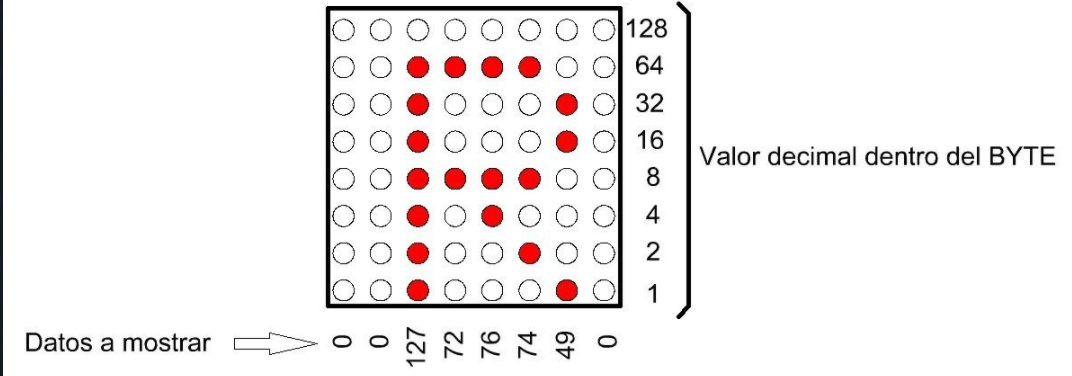
\includegraphics[width=12cm]{decbin.png}
    \centering
    \caption{Paso de binario a decimal}
    \label{decbin}
    \end{figure}
    
Con el vector expresado de esta forma, es más sencillo de llevar el proceso, ya que los números decimales se puede identificar mucho más rápido los errores a la hora de imprimir.

\section{Proceso de montaje}\label{montaje}
Como se comentó en la sección \textbf{\ref{analisis}}, para el montaje del hardware se van a utilizar 8 circuitos integrados conectados entre sí. Donde el mecanismo usado para interconectar los, es que el pin de entrada SER del segundo integrado, se conecta con el pin de  salida  QH' del anterior integrado, formando así una cominucación en serie entre los integrados. Tal como se muestra en la siguiente figura (\textbf{\ref{inter}}).

    \begin{figure}[h]
    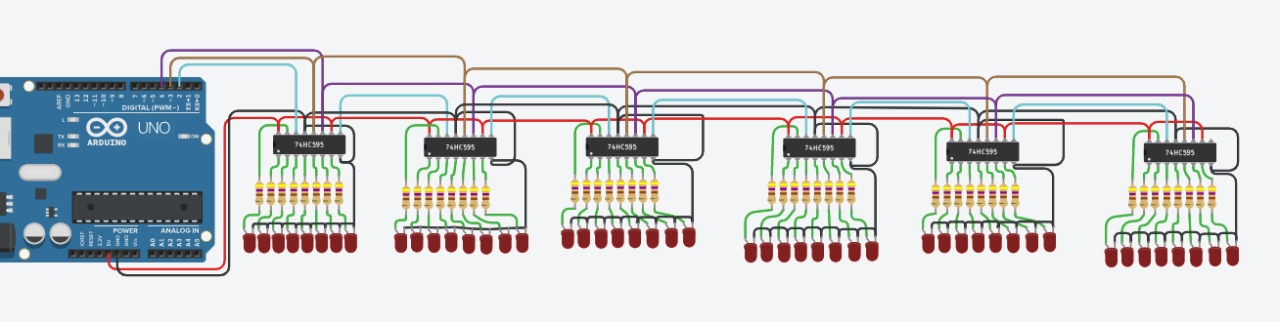
\includegraphics[width=14cm]{inter.jpeg}
    \centering
    \caption{Interconexión de integrados}
    \label{inter}
    \end{figure}

Se ha conectado 8 leds por cada circuito integrado (74HC595) donde cada configuración por CI representa una fila de nuestra matriz 8X8 de LEDs. 
Lo que se hace es conectar el terminal positivo (ánodo) de un LED en serie con una resistencia (470 ohm) por cada salida Qi de los CI (desde Qa hasta Qh),  y la salida Qh’ se interconecta con la entrada SER del siguiente circuito integrado.Por otra parte, los terminales negativos que quedan libres en cada LED se interconectan y son enviados a GND (tierra común), este proceso se repite por cada CI  hasta tener una configuración de 8 circuitos integrados y se acomoda cada fila una debajo de la otra para formar una matriz 8x8 de Leds tal como se muestra en la figura (\textbf{\ref{montaje5}}).


    \begin{figure}[h]
    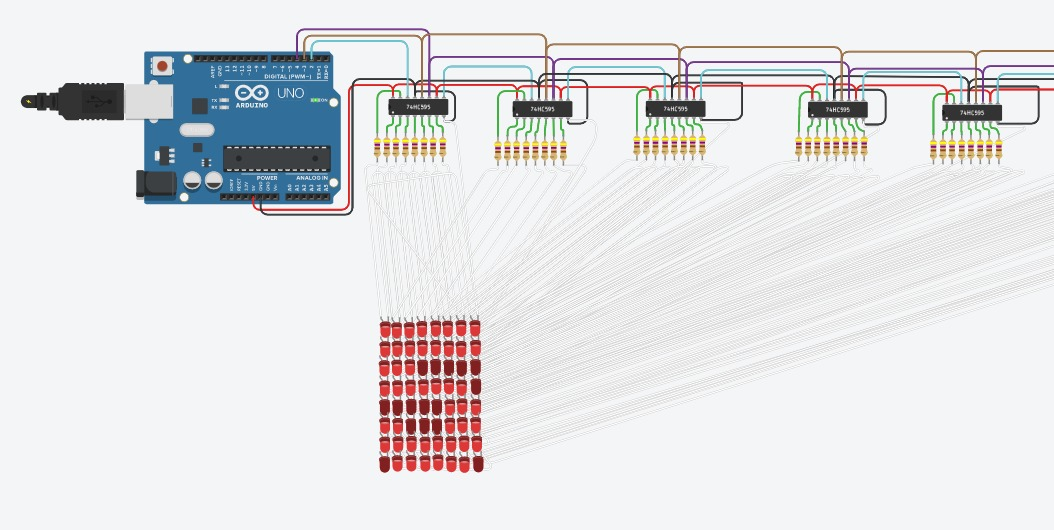
\includegraphics[width=14cm]{montaje5.jpeg}
    \centering
    \caption{Matriz de LEDs funcionando}
    \label{montaje5}
    \end{figure}
    
Cabe resaltar que para este primer prototipo se realiza el montaje y la interconexión de los componentes en el aire por facilidad y también para  obtener los primeros resultados de prueba. En los siguientes prototipos se mejorará el montaje para organizar más el circuito.\\


Para poder mostrar el número 5 en la matriz de LEDs , se debe programar el Arduino.A continuación, se presenta el código, que permite realizar la accion mostrada en la figura(\textbf{\ref{montaje5}}).


\begin{lstlisting}[language=arduino, label=print5]

cconst int SER = 2;
const int RCLK = 3;
const int SRCLK = 4;


char TECLA;

void ledon(int);

void prueba();

void setup()
{
  
  
  Serial.begin(9600);
  
  pinMode(SER , OUTPUT);
  pinMode(RCLK , OUTPUT);
  pinMode(SRCLK , OUTPUT);
 
  digitalWrite(SER , 0);
  digitalWrite(RCLK , 0);
  digitalWrite(SRCLK , 0);
 
  
  prueba1(); // Muestra el patron 5 
  
}

  
void loop(){

}


void ledOn(int n){
  
  	/*
    
    Funcion que enciende una fila del arreglo de LEDS
    segun n
    
    El parametro de entrada (n) es un entero que se convierte
    a binario para generar datos a la entrada SER

    
    */
    int b;
  	for (int i = 0 ; i < 8 ; i++){
    b = n%2;
    n = n/2;
    
     //[paso 1]
    digitalWrite(SER ,b);

    // [Paso 2] 
    digitalWrite(SRCLK , 0);
    digitalWrite(SRCLK , 1);
    digitalWrite(SRCLK , 0);

    // [Paso 3]
    digitalWrite(RCLK , 0);
    digitalWrite(RCLK , 1);
    digitalWrite(RCLK , 0);
  }
}


void prueba1(){
  
    /* Funcion que muestra el numero 5 en un patron de LEDS*/
  
  int p1[8] = {126,255,199,7,254,224,255,255};
  
  for (int k = 0; k < 8; k++){
    ledOn(*(p1+k));
  }
}


void verificacion(){ 
  
  /* Funcion que verifica que todos 
  los LEDS esten encendidos*/
  
  int p2[8] = {255,255,255,255,255,255,255,255};
  
  for (int k = 0; k < 8; k++){
    ledOn(*(p2+k));
  }
}

\end{lstlisting}

Donde se puede apreciar que tiene 2 funciones principales.

\begin{itemize}
    \item \textbf{ void ledOn()}: Función encargada de encender una fila del arreglo de LEDs , a partir del parámetro de entrada \textbf{n} el cual es un número entero que es convertido a binario para generar el arreglo que será procesada por la entrada SER.
    \item \textbf{void verificacion()}:Función la cual le permitirá al usuario verificar que todos los LEDs que están conformando la matriz 8x8 estén funcionando correctamente  y así no haya algún tipo de inconveniente al momento de generar el patrón que el usuario desee formar con los LEDs. Para esto básicamente se debe encender los 64 leds y así cerciorarce de que  cada uno está trabajando.
    
\end{itemize}

\begin{lstlisting}[language=arduino, label=pruebaON]
void verificacion(){ 
  
  /* Funcion que verifica que todos 
  los LEDS esten encendidos*/
  
  int p2[8] = {255,255,255,255,255,255,255,255};
  
  for (int k = 0; k < 8; k++){
    ledOn(*(p2+k));
  }
}
\end{lstlisting}

Por ejemplo para el código \ref{pruebaON}, se crea un arreglo tipo entero de 8 posiciones donde cada posición tiene almacenado un número decimal el cual representa una de las 8 filas de la matriz de leds, en este caso tenemos el número decimal 255 en las 8 posiciones del arreglo p2[8], ya que este número al convertirlo a binario con la función ledOn  representa el número binario 11111111(lo cual significa que se tiene encendidos los 8 LEDs de esa fila) y así sucesivamente se realiza este proceso con el ciclo For 8 veces, al  terminar este ciclo se tiene encendidos los 8 leds de las 8 filas, el cual representa la matriz 8x8 de LEDs encendidos todos.\\

Este proceso es de vital importancia dado que es la base de como se va a imprimir todas las letras y el patrón que ingrese el usuario.\\

    \begin{figure}[h]
    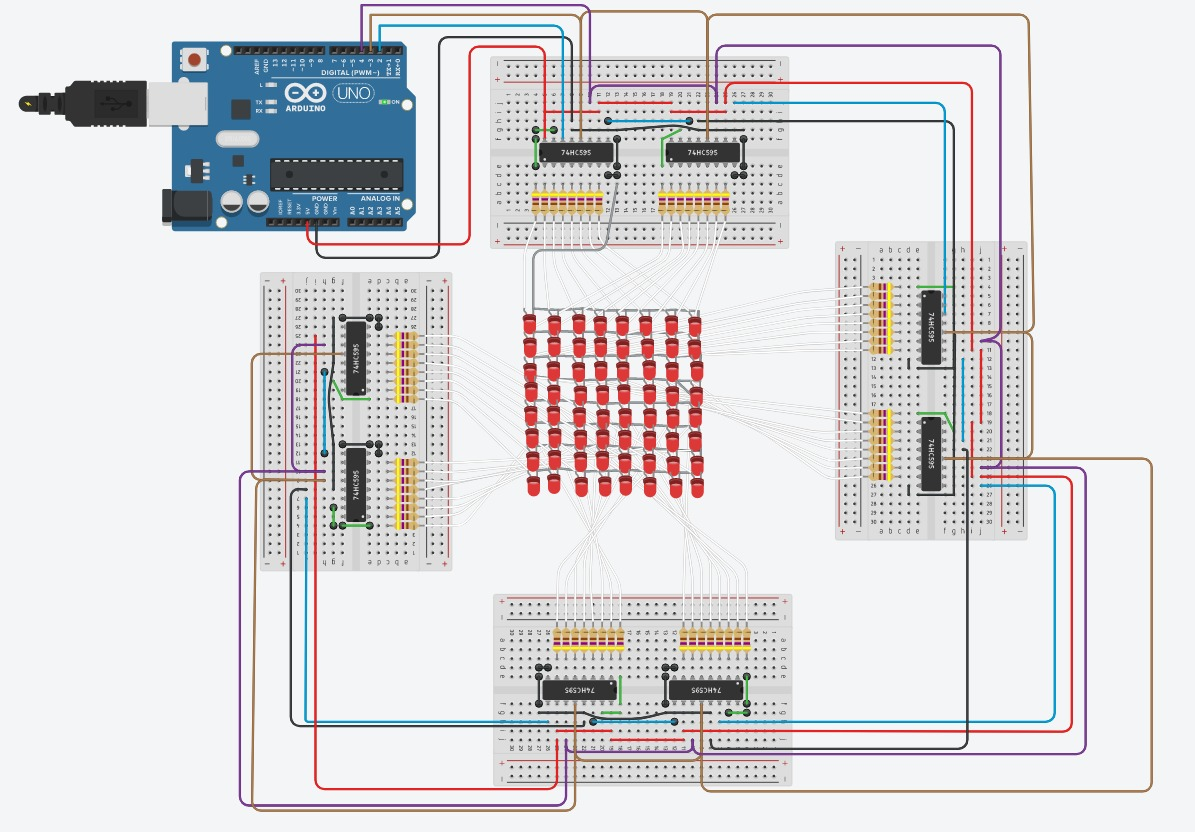
\includegraphics[width=11cm]{FullMontaje.jpeg}
    \centering
    \caption{Montaje final hardware}
    \label{circuito}
    \end{figure}
    
En la figura ( \textbf{\ref{circuito}} ) se muestra como se modificó el montaje de Tinkercad, ya que anteriormente se tenía el montaje en el aire, esto porque es más fácil visualizar cualquier error de falla de conexión. No obtasnte, ya pusimos a prueba el sistema tanto en programación como en hardware. Entonces ya se realizó el montaje en tablas de prueba o protoboard, donde cada una tiene 2 integrados para mayor orden.\\

Se puso en funcionalidad las lineas de código que hacen interactuar al usuario con el Monitor Serial. En la figura ( \textbf{\ref{solicitud}} ) se muestra que se va a ingresar el patrón HEY, con un delay de dos segundos. En la figura ( \textbf{\ref{ejecucionH}} ) los leds muestran una configuración mostrando el patrón Y, que es el ultimo patrón de la secuencia.\\

   \begin{figure}[h]
    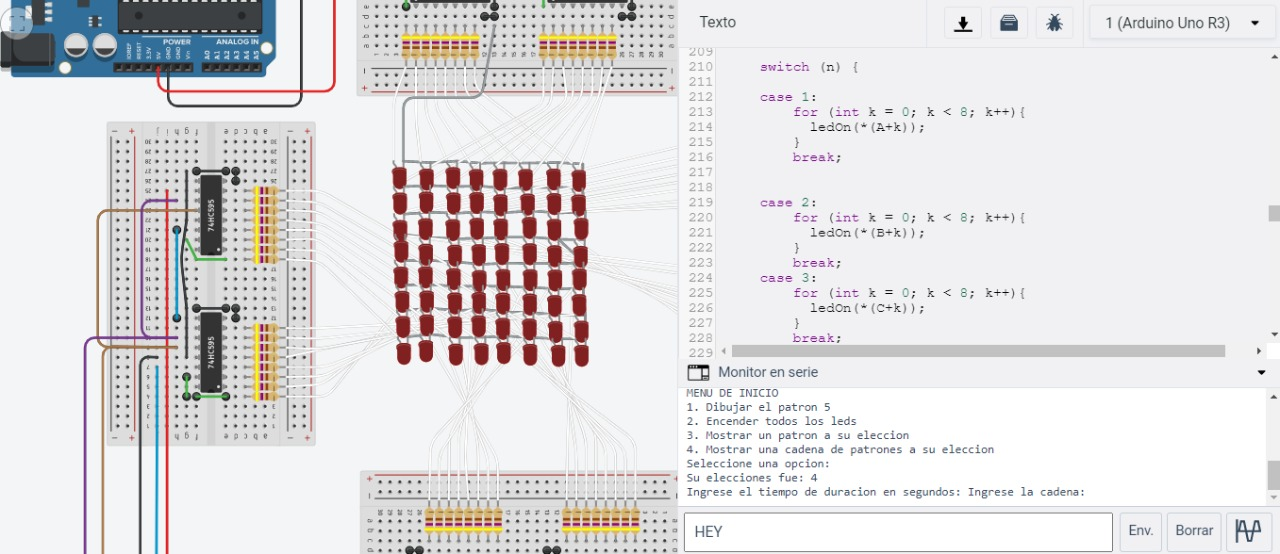
\includegraphics[width=11cm]{montaje6.jpeg}
    \centering
    \caption{Solicitud de información por Monitor en Serie}
    \label{solicitud}
    \end{figure}
    
       \begin{figure}[h]
    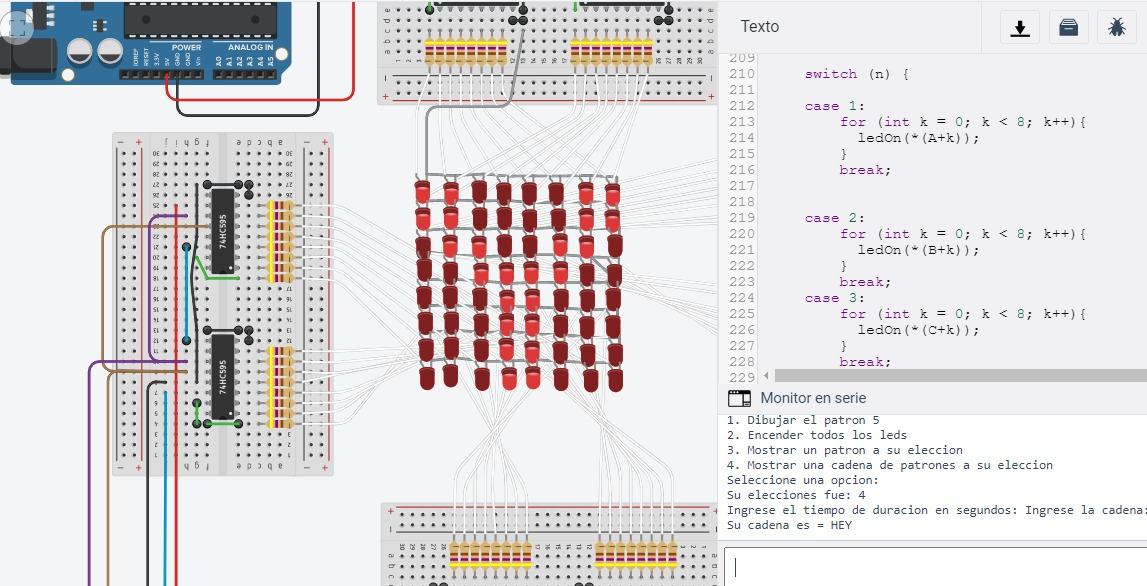
\includegraphics[width=11cm]{montaje7.jpeg}
    \centering
    \caption{Finalización de ejecucion con la entrada HEY}
    \label{ejecucionH}
    \end{figure}
    
    El siguiente código muestra el usuario va a interactuar con la consola, se observa que la varaible \textit{ENTRADA} es la que decide a que parte del programa desea ir, entre las opciones está, \textbf{1.} Verficiar el \textit{patron 5},\textbf{ 2.} Verificar si todos los Leds están enceididos,\textbf{ 3.} Ingresar un carácter por teclado para mostrar en el arreglo de leds,\textbf{ 4.} Ingresar una cadena de cáracteres para mostrar en  el arreglo de leds, cada condicional, según la entrada, lleva a otras instrucciones que son quienes ejecutan las procesos sobre el funcionamiento del arreglo\\


\begin{lstlisting}[language=arduino, label=pruebaON]
void verificacion(){ 
    while(Serial.available()==0){}
    
  int ENTRADA = Serial.parseInt(); // lee un entero 
  Serial.print("Su elecciones fue: ");
  Serial.println(ENTRADA);
  
  
  
  if (ENTRADA == 1){
    // Ingresa a verificar el patron 5 
    prueba1();
  }
  
  else if(ENTRADA == 2){
    // Ingresa a realizar la verifiacion
    // que todos los LEDS esten encnendidos
    
    verificacion();
  }
  
  else if(ENTRADA == 3){
   
    Serial.println("");

    // pedir al usuario un caracter para ser
    // visualizado
    
    Serial.println("Ingrese un caracter para mostrar el patron: ");
    while(Serial.available()==0){}
    
  	int ENTRADA3 = Serial.read(); // lee ascii 
  	//Serial.println("Su caracter ingresado fue: ");
  	//Serial.println(ENTRADA3);
    
    imagen(ENTRADA3); // A - > 65  caso 1 = A 65-64 -> 1 

    
  }
  
  if(ENTRADA == 4){
    // Pide al usuario que le ingrese una palabra para ser
    // mostrada secuencialmente, el tiempo entre patron y 
    // patron lo define el usuario y la variable se llama
    // TIEMPO
	Serial.println("");
    Serial.print("Ingrese el tiempo de duracion en segundos: ");
    while(Serial.available()==0){}
    int SEGU = Serial.parseInt(); 
  
	publik(SEGU);
    
  }
}
  }
}
\end{lstlisting}

\section{Problemas obtenidos}\label{problem}
En esta sección se habla sobre los errores y problemas que se tuvo a la hora de realizar el desafío, con el fin de ponerlos al conocimiento del estudiantado para aprender a trabajar y solucionar en momentos de crisis, o bajo presión.

En primer lugar, el problema más notable que se obtuvo está relacionado con los repositorios, donde al momento de crear un repositorio compartido el día domingo 18 de abril del 2021,se subieron unos documentos de prueba para verificar el uso de esta herramienta. Tiempo después se intentó  realizar commits, pero siempre se encontraban problemas con la sincronización de repositorios, arrojando errores respecto realizar un git pull,ver figura (\textbf{\ref{repoerror}}).

    \begin{figure}[h]
    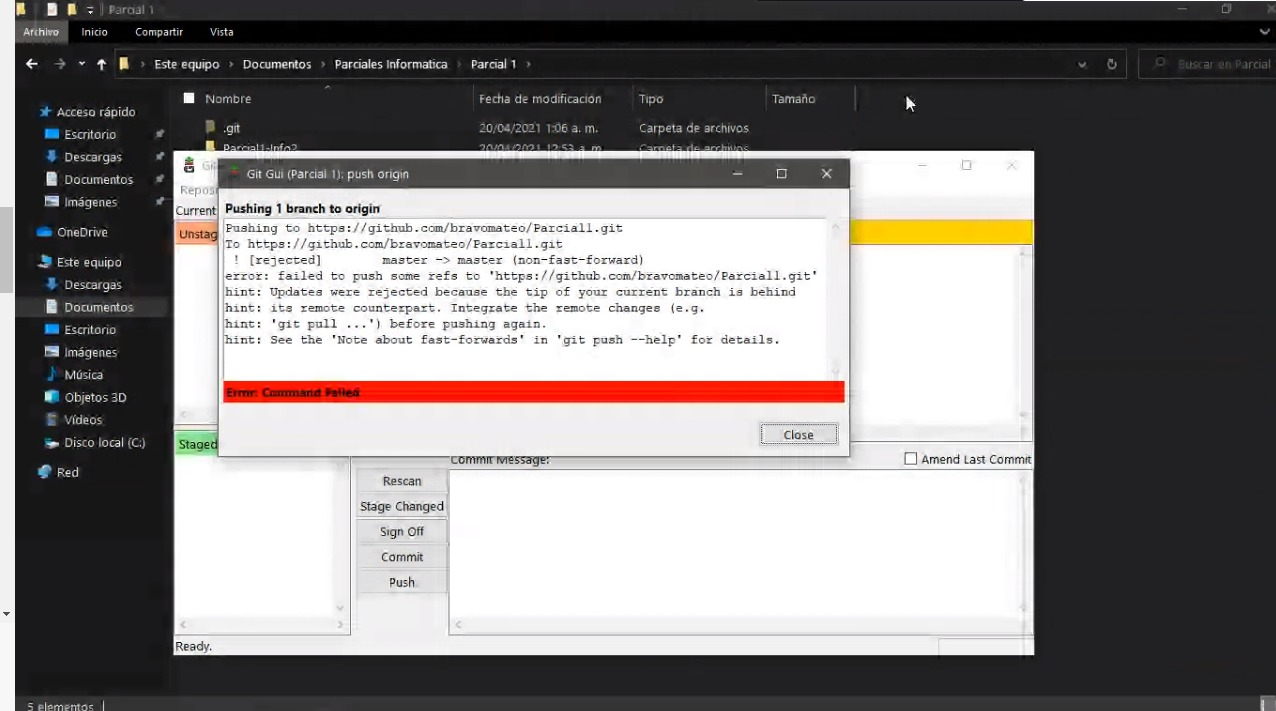
\includegraphics[width=15cm]{Error1.jpeg}
    \centering
    \caption{Error de repositorios}
    \label{repoerror}
    \end{figure}
    
Se intentó arreglar este error buscando en diversas fuentes, distintas soluciones, utilizando comandos tales como, git pull remote, git fetch, git merge, incluso se optó por borrar a los contribuidores con el fin de que no intervinieran más, pero la respuesta siguió siendo negativa,razón por la que se dejó de lado el repositorio\\ \url{https://github.com/bravomateo/Parcial1.git} . Dado esta circuntancia , se tomó la iniciativa de crear un nuevo repositorio el día lunes 19 de abril sin tener ningun colaborador , para evitar tener este problema y poder continuar con el desarrollo del reto.Este problema del repositorio tuvo un fuerte impacto porque tuvo un costo de mucho tiempo.\\




\bibliographystyle{IEEEtran}
\bibliography{references}

\end{document}
